\subsection{What is deep learning?}
Deep Learning is a subclass of machine learning, where instead of using space transformations it uses multiple non-linear transformations to progressively extract higher level features from input data. This set of non-linear transformations is called Neural Network. The proper transformations are found in a process called 'training' which is just a Machine Learning environment expression for optimization using Gradient Descent.  

In image recognition problems Neural Network (NN) takes pixel values as input data, apply non-linear transformations, and as a result return a vector of probability distribution over a set of classes.


\subsection{How is deep learning used in Face Recognition Systems?}


The face recognition algorithm used in 'Deep Face Recognition' [6] works very similar to the classic image recognition algorithm. As an input data it uses a picture of a face, it propagates it through a NN and as a result it returns a vector of probabilities. (See Figure 1). Then a Face Recognition System (FRS) finds a class with the highest probability value and that is the predicted persons identity. 

\begin{figure}[!ht]
\centering
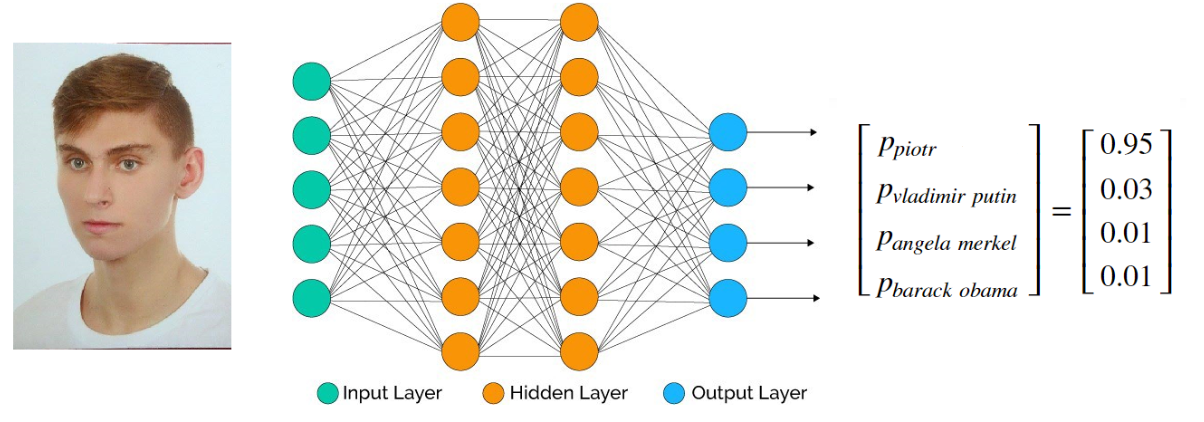
\includegraphics[width=0.9\textwidth]{Images/face-recognition.png}
\caption[]{FRS returns distribution of probabilities over set of faces}
\end{figure}